%%%%%%%%%%%%%%%%%%%%%%%%%%%%%%%%%%%%%%%%%%%%%%%%%%%%%%%%%%%%%%%%%%%%%%%%%%%%%%%%%%
% ICA 2019 template with improvements by Prof. Will D'Andrea Fonseca - 31/05/2019
%%%%%%%%%%%%%%%%%%%%%%%%%%%%%%%%%%%%%%%%%%%%%%%%%%%%%%%%%%%%%%%%%%%%%%%%%%%%%%%%%%
\section{\uppercase{Introduction}}

Use this document as a guide when writing your paper. Wherever possible, use the styles that have been defined in this document. This and other paragraphs in this document were formatted with the ``Paragraph'' style.

Only manuscripts written in the English language will be accepted for inclusion in the Proceedings. The number of pages shall not exceed 8 --- except for plenary and keynote speaker. The Technical Program Committee reserves the right to reject any manuscript considered inappropriate for the Proceedings, even if the abstract was previously accepted.

The exclusive use of SI units is strongly recommended. If the English conventional system of units is used, the English equivalents shall be inserted in parentheses following the metric values , for example 25.4 mm (1 in).

%%%%%%%%%%%%%%%%%%%%%%%%%%%%%%%%%%%%%%%%%%%%%%%%%%%%%%%%%%%%%%%%%%%%%%%%%%%%%%%
\section{\uppercase{Manuscript format}}

%%%%%%%%%%%%%%%%%%%%%%%%%%%%%%%%%%%%%%%%%%%%%%%%%%%%%%%%%%%%%%%%%%%%%%%%%%%%%%%
\subsection{Margin settings}

The A4 standard paper size will be used for all Conference papers with all margins set to 25~mm. This setting and other settings are automatically set if this template is used in Microsoft Word.

Please do not insert any page numbers. Do not include anything in the headers or footers except for the footnotes for e-mail addresses on the first page of the manuscript.

%%%%%%%%%%%%%%%%%%%%%%%%%%%%%%%%%%%%%%%%%%%%%%%%%%%%%%%%%%%%%%%%%%%%%%%%%%%%%%%
\subsection{First page heading}

The logo for Conference papers shall appear centred at the top of the first page. The logo does not appear on subsequent pages. When you are using this document as a template, the logo has already been inserted into the header section for the first page. 

\clearpage
%%%%%%%%%%%%%%%%%%%%%%%%%%%%%%%%%%%%%%%%%%%%%%%%%%%%%%%%%%%%%%%%%%%%%%%%%%%%%%%
\subsection{Title of paper}

The paper title shall use the Arial 14-point bold font and shall not exceed 20 words. Except for proper nouns, only the first word of the title is capitalized. Center the title as shown above. Use the pre-defined style ``Title of paper''.

%%%%%%%%%%%%%%%%%%%%%%%%%%%%%%%%%%%%%%%%%%%%%%%%%%%%%%%%%%%%%%%%%%%%%%%%%%%%%%%
\subsection{Author information}

Author information shall be inserted below the title and centred using the above example as a guide. The font for author names is Times New Roman, 11-point regular. Use the pre-defined style ``Authors''. For each author, provide the given name(s) followed by the FAMILY NAME in upper case. Separate multiple author names by a semi-colon.

Place authors' institutions and countries below the list of authors' names using Times New Roman 10-point regular font (pre-defined style ``Affiliation''). If there are more than three authors, continue adding authors and their affiliations according to the examples on the first page of this template.
Optional: Put the authors' e-mail addresses at the bottom of the first page by using the ``Footnote'' option of Microsoft Word and setting this option to `on page' not `end of document'.

%%%%%%%%%%%%%%%%%%%%%%%%%%%%%%%%%%%%%%%%%%%%%%%%%%%%%%%%%%%%%%%%%%%%%%%%%%%%%%%
\subsection{Headings}

The Arial font is specified for all headings. Sans-serif fonts such as Helvetica may be substituted for Arial if necessary. All headings shall be flush left. Use a tab --- not a space --- between the heading number and the first word of the heading. The first tab stop is 1 cm from the left hand edge of the text

Major level 1 headings shall be 12-point upper case Arial bold font and numerically ordered. Use the pre-defined style ``1. Major Headings.'' The spacing before the heading is 12-point with 1-point after.

Level 2 subheadings shall be in 10.5-point Arial bold type with upper and lower case. Use the pre-defined style ``1.1 Subheadings.'' The spacing before the subheading is 6-pt with no space after. 

A level 3 heading has been defined, but is not expected to be widely used. If required, use the pre-defined style ``1.1.1 Third headings.'' which uses 10.5-point Arial bold type with upper and lower case. The space before the third heading is 3-pt with no space after.

As shown in this document, major headings shall be numerically ordered as 1, 2, etc. while subheadings are numerically ordered as 2.1, 2.2, etc. If finer subheadings are required they shall be numbered as 2.6.1, 2.6.2, etc.

%%%%%%%%%%%%%%%%%%%%%%%%%%%%%%%%%%%%%%%%%%%%%%%%%%%%%%%%%%%%%%%%%%%%%%%%%%%%%%%
\subsection{Main body}

The font for the main body of text is 10.5-point, regular Times New Roman or Times medium. If these fonts are not available, a similar serif font may be substituted. The first line of a paragraph is indented by 0.5 cm. Use the pre-defined style ``Paragraph'' for the text of the main body of a paper.

%%%%%%%%%%%%%%%%%%%%%%%%%%%%%%%%%%%%%%%%%%%%%%%%%%%%%%%%%%%%%%%%%%%%%%%%%%%%%%%
\subsection{Graphics and tables}

%%%%%%%%%%%%%%%%%%%%%%%%%%%%%%%%%%%%%%%%%%%%%%%%%%%%%%%%%%%%%%%%%%%%%%%%%%%%%%%
\subsubsection{Figures and photographs}

Incorporate all graphics, charts, tables, illustrations, photos, etc. directly into your manuscript shortly after their first mention. An example of the preferred layout of a graphic is shown in Figure \ref{fig:figure1}.

The graphic was centred on the page using the pre-defined ``Style of Figure''. The figure has a caption label beneath the graphic and in 10.5-point Times New Roman, and centred by using the pre-defined style ``Caption.''

If your paper includes photographs, you need to reduce the dimensions of each image and place the reduced image in the text after first mention. Do not use high-resolution pictures, since that is likely to increase the size of your final PDF file. A resolution of 300 dots per 25 mm should be sufficient for the purpose of most papers. Ensure that all images use the RGB not CYMK colour space.

\begin{figure}[H]
\centering
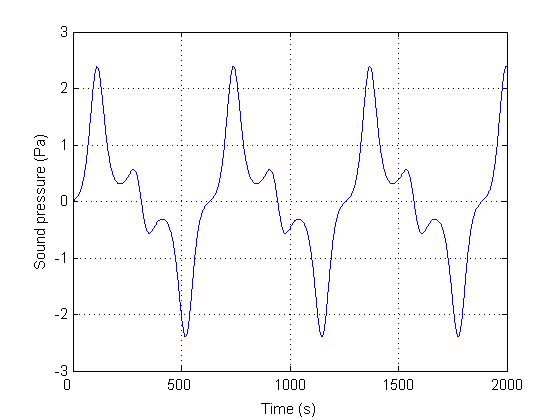
\includegraphics[width=0.75\linewidth]{fig/figure1.png}
\caption{This is a caption for the figure}
\label{fig:figure1}
\end{figure}

%%%%%%%%%%%%%%%%%%%%%%%%%%%%%%%%%%%%%%%%%%%%%%%%%%%%%%%%%%%%%%%%%%%%%%%%%%%%%%%
\subsubsection{Tables}

An example of a table is as follows (Tables~\ref{tab:table1} and \ref{tab:table2}).

\begin{table}[!ht]
\caption{Physical parameters of liquids}
\label{tab:table1}
\centering \renewcommand{\arraystretch}{2}
\begin{tabular}{cccc}
\hline 
Liquid & Molecular formula & Density, g/cm$^3$ & Sound speed, m/s \\ \hline
Benzene	& C$_6$H$_6$ &	0.87 & 1295\\
Acetone &	C$_3$H$_6$O &	0.79 &1170\\
Water	& H$_2$O & 1.0 & 1500\\ \hline
\end{tabular} 
\end{table}

\begin{table}[H]
  \centering 
  \caption{A second example of table}
	\fontsize{11}{12}\selectfont 
    \begin{tabular}{C{3.8cm} | C{3.8cm}}
    \toprule
		\SetRowColor{LightOrange}
    \textbf{ xxx } & \textbf{yyy} \\
	  \midrule
		10 & 3120\\
		\rowcolor[gray]{.95} 40	& 2555\\
		50 & 1100\\
    \bottomrule
    \end{tabular}
    \label{tab:table2}
\end{table}%

Tables are centred on the page. The caption is placed just above the table and uses the pre-defined style ``Caption.''

%%%%%%%%%%%%%%%%%%%%%%%%%%%%%%%%%%%%%%%%%%%%%%%%%%%%%%%%%%%%%%%%%%%%%%%%%%%%%%%
\subsection{Equations}

Equations shall be typeset (using the Microsoft Equation Editor if using MS Word) as follows

\begin{equation}
E = mc^2 \,,
\label{eq:equation1}
\end{equation}
%
where $E$ is... etc. When referring, it is possible to use Equation~\eqref{eq:equation1}.

The equation is set into a two-column 160-mm-wide table where the left-hand 150-mm-wide column contains the equation, and the right-hand column the equation number enclosed in parentheses. The equation is centred within the cell, and the equation number is vertically centred to align with the equation. Use the 10.5 point Times New Roman font. Fractions in a simple equation are best shown on one line with the numerator and denominator separated by a solidus [/], not built-up with a numerator above a denominator. However, more complex equations should use equation editor or equivalent software.

%%%%%%%%%%%%%%%%%%%%%%%%%%%%%%%%%%%%%%%%%%%%%%%%%%%%%%%%%%%%%%%%%%%%%%%%%%%%%%%
\subsection{References}

In the text, indicate references between brackets, e.g., ``...noise sources can be identified \cite{beranek,adaptive:1985}...'' and ``... action can be taken as reported by Embleton \cite{tutorial:1996}''. References to conference articles are shown by references \cite{active:1994, stinson:1996, Fonseca-2013}. The required reference style is Thomson Reuters Endnote's ``Vancouver'' reference style. Examples of this reference style are given in the list of references. Users of zotero (free bibliography software for Firefox) should refer to \href{http://www.zotero.org/styles/?q=vancouver}{http://www.zotero.org/styles/?q=vancouver}.

Please use the pre-defined style ``References'' for the references. All but the first line of each reference are indented 0.5 cm. The font is 10.5 point Times New Roman.

%%%%%%%%%%%%%%%%%%%%%%%%%%%%%%%%%%%%%%%%%%%%%%%%%%%%%%%%%%%%%%%%%%%%%%%%%%%%%%%
\section{\uppercase{Other important information}}

%%%%%%%%%%%%%%%%%%%%%%%%%%%%%%%%%%%%%%%%%%%%%%%%%%%%%%%%%%%%%%%%%%%%%%%%%%%%%%%
\subsection{Intellectual property}

Authors must obtain permission from the intellectual property holders before publishing or reproducing figures, images or other intellectual property in their manuscript. An acknowledgement that such permission has been obtained from the intellectual property holders must be included in the manuscript.

%%%%%%%%%%%%%%%%%%%%%%%%%%%%%%%%%%%%%%%%%%%%%%%%%%%%%%%%%%%%%%%%%%%%%%%%%%%%%%%
\subsection{Submission of papers}

All papers shall be submitted on-line as MS-Word files (*.doc or *.docx) or as unprotected PDF files (Adobe Portable Document Format) via the Conference website \url{www.isra2019.eu}. Use the reference number and password given in the e-mail sent after the submission of your abstract. The size of the paper file shall not exceed 10-megabytes. Given the large numbers of papers expected for this conference, the Secretariat does not have the resources to typeset or to proofread the individual papers. Please review your paper carefully for format, spelling, grammar, punctuation, and technical content. Your paper will be placed into the Proceedings just as received. Any paper that varies from the format presented in this template will be returned to the author(s) for re-formatting using the guidance of this template. Only papers conforming to the template guidelines will be included in the proceedings.

The deadline for submission of the complete manuscript is July 15, 2019. However, the deadline for manuscripts seeking peer review is July 1, 2019. Your paper can only be accepted if the PDF file is uploaded via the Conference Website. The corresponding author (who submitted the abstract) will be notified of receipt of the paper by e-mail. If you do not receive an e-mail notifying you of the receipt of your paper within 24 hours of your paper submission, please notify the editor of this fact by e-mail to \href{mailto:isra2019@conforg.fr}{isra2019@conforg.fr}.

%%%%%%%%%%%%%%%%%%%%%%%%%%%%%%%%%%%%%%%%%%%%%%%%%%%%%%%%%%%%%%%%%%%%%%%%%%%%%%%
\subsection{Mandatory registration of authors}

An invited or contributed paper may be part of the Conference program and proceedings only if a registration fee (Regular Participant or Student) has been paid by the deadline for the paper submission for the Proceedings. One registration fee is valid only for one paper. If the same author submits more than one paper, the ``Additional paper'' fee shall be paid for each additional paper submitted (exception: multiple invited contributions).

%%%%%%%%%%%%%%%%%%%%%%%%%%%%%%%%%%%%%%%%%%%%%%%%%%%%%%%%%%%%%%%%%%%%%%%%%%%%%%%
\section{\uppercase{Conversion to portable document format (PDF)}}

%%%%%%%%%%%%%%%%%%%%%%%%%%%%%%%%%%%%%%%%%%%%%%%%%%%%%%%%%%%%%%%%%%%%%%%%%%%%%%%
\subsection{Embedding fonts}

One of the most common problems related to conversion to PDF format is failure to embed fonts in the document created by a word processor program. If fonts are not embedded, the PDF conversion program does its best to select fonts that match the original document, but the appearance of the PDF file may not be what is intended.

To embed fonts in a Microsoft Word file, go to ``Word Options.'' Then click on ``Save'' and check the box ``Embed fonts in file.'' You can reduce the size of the MS Word file by also checking ``Embed only the characters used in the document (best for reducing file size)'' and ``Do not embed common system fonts''. Other word processing programs may have similar options. 

If using Adobe Acrobat to convert the document to PDF format, go into Properties in the print dialogue box and untick ``Rely on system fonts only: do not use document fonts''.

%%%%%%%%%%%%%%%%%%%%%%%%%%%%%%%%%%%%%%%%%%%%%%%%%%%%%%%%%%%%%%%%%%%%%%%%%%%%%%%
\subsection{Inspecting your PDF file}

Carefully inspect your PDF file before submission to be sure that the PDF conversion was done properly and that there are no error messages when you open the PDF file. Common problems are: missing or incorrectly converted symbols especially mathematical symbols, failure of figures to reproduce, and incomplete legends in figures. Identification and correction of these problems is the responsibility of the authors.

%%%%%%%%%%%%%%%%%%%%%%%%%%%%%%%%%%%%%%%%%%%%%%%%%%%%%%%%%%%%%%%%%%%%%%%%%%%%%%%
\section{\uppercase{Conclusions}}

The section before the references is normally called CONCLUSIONS, SUMMARY, or FINAL REMARKS, where the authors describe the most-relevant findings of the work\footnote{This is a footnote.}.

%%%%%%%%%%%%%%%%%%%%%%%%%%%%%%%%%%%%%%%%%%%%%%%%%%%%%%%%%%%%%%%%%%%%%%%%%%%%%%%
\section*{\uppercase{Acknowledgements}} \addcontentsline{toc}{section}{Acknowledgements}

Authors may acknowledge financial or other forms of support in this Section. All acknowledgements shall be placed after Conclusions and before References. Numerically ordering is not necessary for the ``ACKNOWLEDGEMENTS'' or ``REFERENCES'' headings, which should use the pre-defined style ``Major without number''.

%%%%%%%%%%%%%%%%%%%%%%%%%%%%%%%%%%%%%%%%%%%%%%%%%%%%%%%%%%%%%%%%%%%%%%%%%%%%%%%
% EOF
